\chapter{Methods}
% This should be 3000 words split with the results
% Probably gonna go for like 2200/800 as you have very few results

% the design of the task

%%%%%%%%%%%%%%%%%%%%%%%%%%
\section{Examining and Bridging the Gap}

% Two alternative forced choice
A typical decision neuroscience task is similar to the dot task discussed in the literature review. That is a discrete perceptual task requiring the subject to discriminate between one of two choices. This type of task can be broadly described as a "two-alternative forced choice" (TAFC) task.

The crux of this thesis was to fit driving to this paradigm; how can the complex task of driving be reduced in complexity to allow for effective modelling of the driver/cyclist interaction without sacrificing the ability to gain true insight into the decision process.


% what makes driving very complicated
% what makes decision tasks very complicated
% How do
%%%%%%%%%%%%%%%%%%%%%%%%%%
\section{Gaining Familiarity with Decision Neuroscience}

%%%%%%%%%%%%%%%%%%%%%%%%%%
\section{Beginning the Task Construction - Psychtoolbox and its Limitations}
% Why Psychtoolbox
Psychtoolbox is a software created to form a bridge between MATLAB and computer display hardware \cite{kleinerWhatNewPsychtoolbox32007}. It allows incredibly control over every pixel on the screen in a precisely timed frame by frame fashion. It is the standard software used within not just the cognitive neural systems lab in UCD but also throughout decision neuroscience research around the world. Furthermore, it builds upon the MATLAB workspace, familiar to UCD engineering students due to extensive use in the undergraduate engineering course.

% Early experimentation, trying to adapt anna's code
% Working with decision neuroscience models, trying to fit Kelly & O'Connell 2013 to a 
At the beginning of the work package it was deemed appropriate that some experience be gained with the Psychtoolbox environment by adapting the model created in \citet{geuzebroekBalancingTrueFalse2023} to the data in \citet{kellyInternalExternalInfluences2013}. This was based on two key assumptions. The first being that the data which was gathered during the latter was similar to that which was expected following the construction of this task. The second being that having experience not only with the general format of the data outputted by the cognitive neuroscience lab but also the structure of the modelling apparatus used.


% Psychtoolbox's limitations
One of the earliest and largest challenges that was faced with the implementation of the decided upon task was Psychtoolbox's inability to handle perspective natively. While it is very capable of accurately drawing a variety of shapes to the screen with precise control over positioning it has no ability to handle the intricacies of camera projection.

\begin{figure}[hbt!]
    \centering
    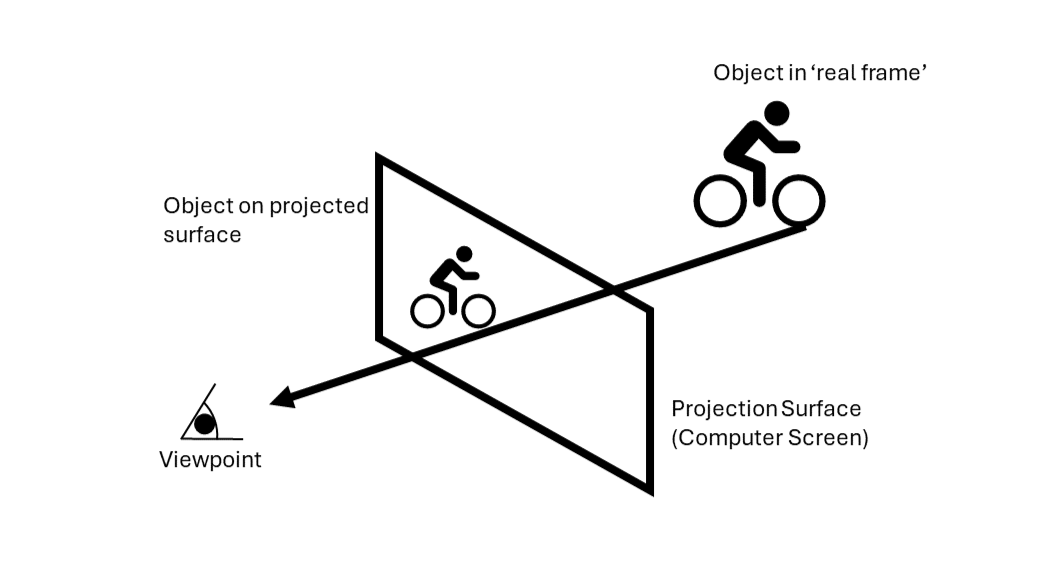
\includegraphics[width=0.75\linewidth]{figures/Projection Diagram.png}
    \caption{Diagram showing the 'real frame' and its projection onto the display screen}
    \label{fig:}
\end{figure}

The early experimentation that took place in this thesis involved trying to draw a box to a screen which could imitate a 'cyclist' on the road as can be seen in figure \ref{fig:EarlyPsychExp}. This experimentation involved the rudimentary projection of a 'real frame' path taken by the cyclist onto a screen. It quickly became clear that the implementation of this projection by calculating the vector mathematics would require vastly more time and knowledge than available. On top of this, limitations within MATLAB's efficiency would have made an implementation impractical. As a result, the task would have to make use of the 

\begin{figure}[hbt!]
    \centering
    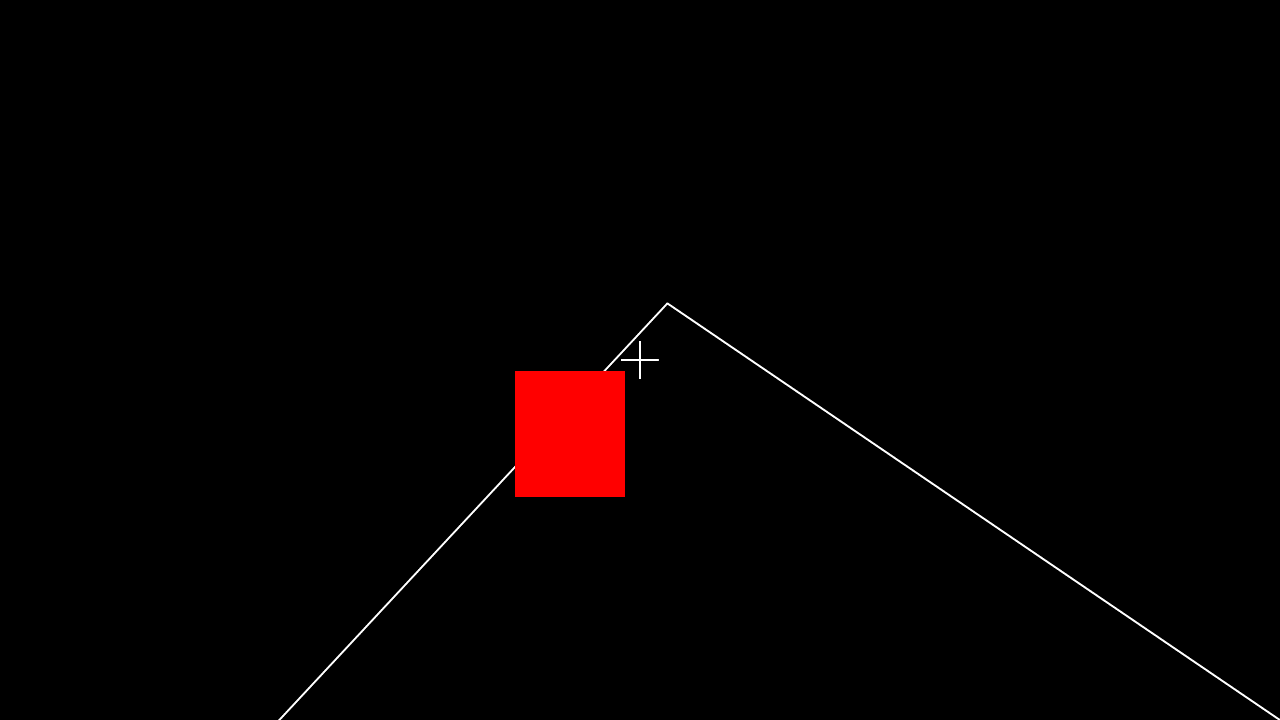
\includegraphics[width=0.45\linewidth]{figures/Slide1.png} \hfill
    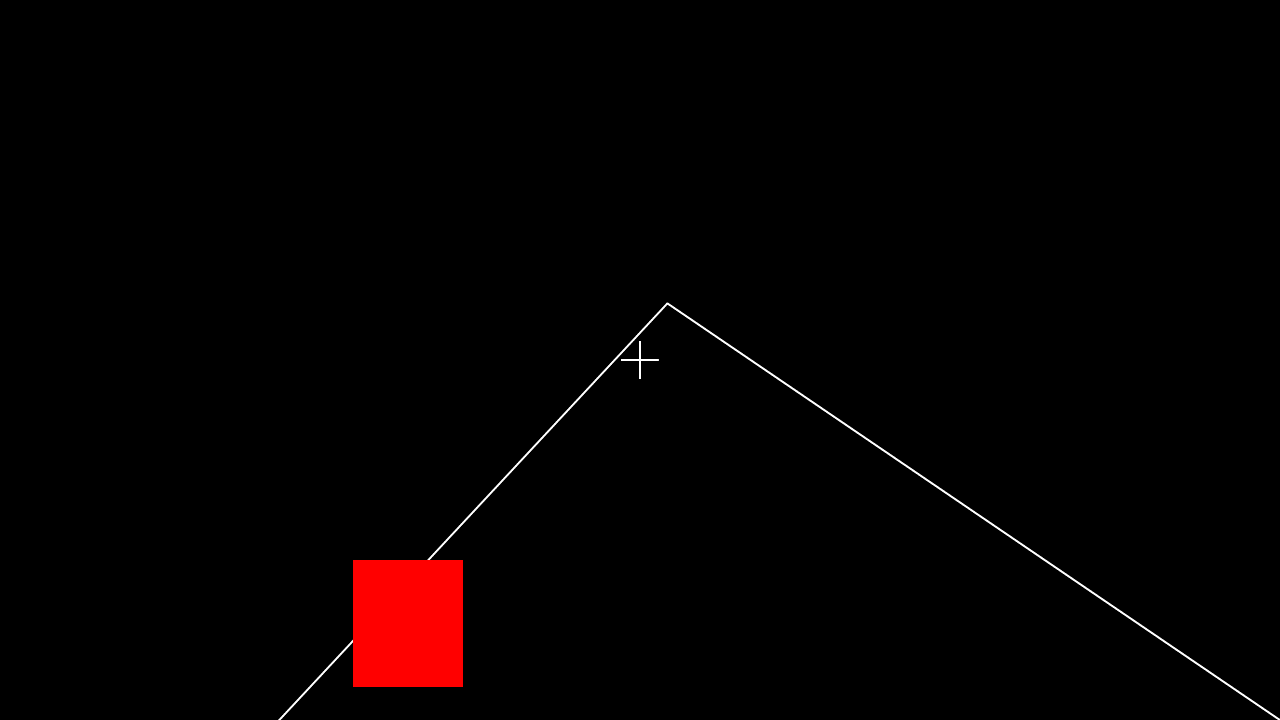
\includegraphics[width=0.45\linewidth]{figures/Slide2.png}
    \caption{The results of early experimentation in Psychtoolbox, a square which appears to move closer to the camera}
    \label{fig:EarlyPsychExp}
\end{figure}

%%%%%%%%%%%%%%%%%%%%%%%%%%
\section{OpenGL and Perspective}
% Talk about OPENGL

% Talk about camera & positioning
\begin{figure}[hbt!]
    \centering
    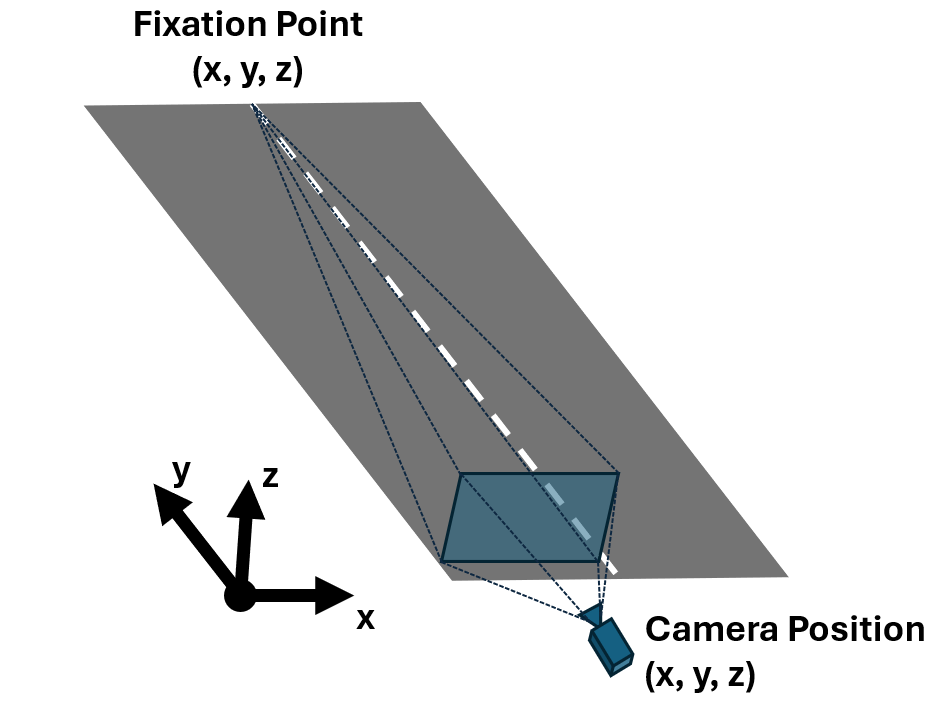
\includegraphics[width=0.45\linewidth]{figures/Camera Positioning.png}
    \caption{Diagram describing how camera positioning is handled within OpenGL}
    \label{fig:CameraPos}
\end{figure}

% Talk about the explainer code

% Talk about the limitations of Psychtoolboxes implementation of openGL

% Talk about what this enabled
% Make particular note of how it enabled the use of units which have 1:1, useful correlation with the physical quantities we are looking to describe
One of the great advantages of this approach was that objects positions, speed and sizes can be described using actual physical quantities. That is opposed to the native Psychtoolbox approach which uses measurements relative to the screen such as pixels. This proved to be of immense import, especially when it came to the implementation of motion, simplifying the complexity of the process significantly.

As the complexity of the task grew it became easier to examine and 

% Talk about the traffic lights here
One dynamic that came up frequently in discussion within the context of the driver/cyclist interaction was the overtaking of a cyclist despite an upcoming red light. Frequently a cyclist will be overtaken at a near distance only to immediately pass on the inside of the overtaking vehicle. Within the realm of computer graphics, a traffic light does not represent an object of immense complexity. However, within the context of the framework of this task it was deemed to be an inappropriate addition. This task was built upon the idea that subjects be shown a continuously varying and pseudo-randomly generated environment. Each level of complexity which gets added to this environment inevitably leads to 

%%%%%%%%%%%%%%%%%%%%%%%%%%
\section{Constructing the Task Frame}
Control over the positioning and movement of objects within the 'real frame' was the primary motivation of the 


\begin{figure}[hbt!]
    \centering
    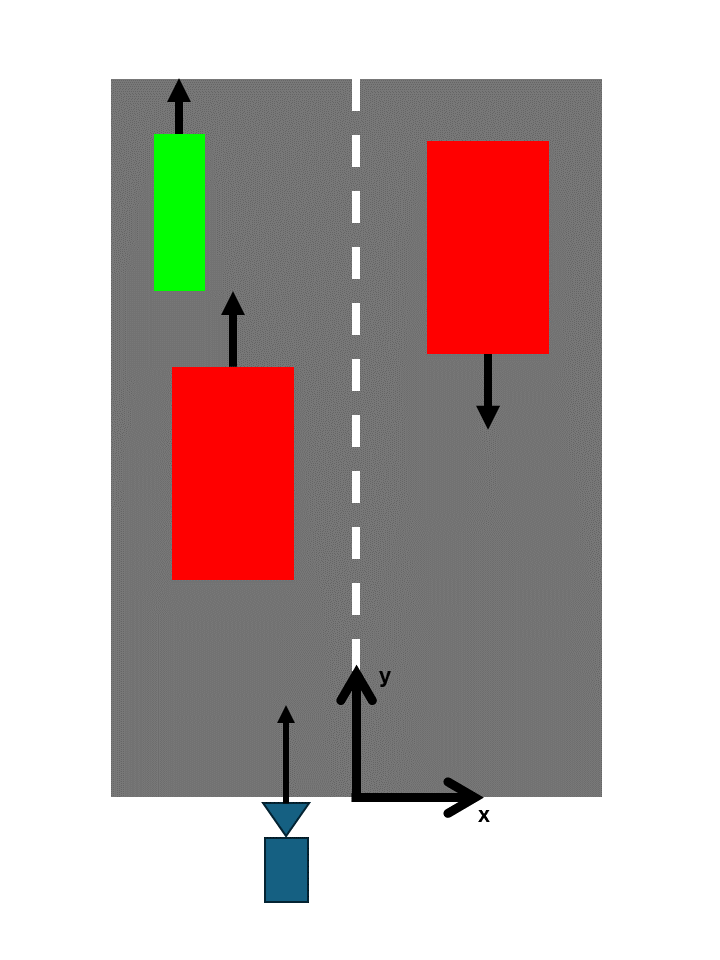
\includegraphics[width=0.45\linewidth]{figures/Frame1.png} \hfill
    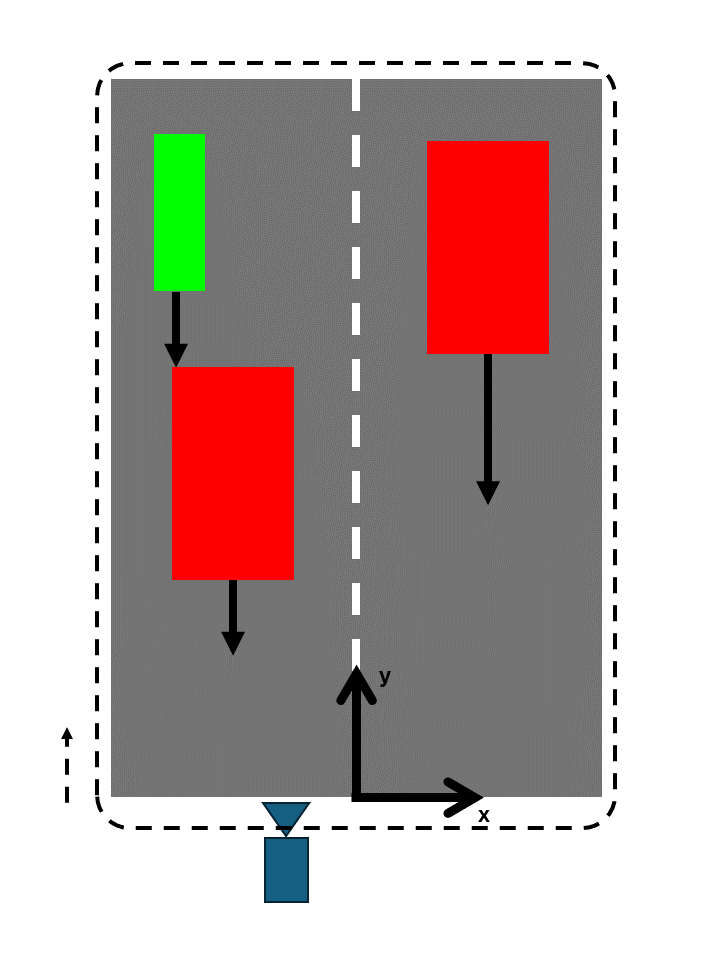
\includegraphics[width=0.45\linewidth]{figures/Frame2.png}
    \caption{The conversion from a 'real frame' of motion to a relative frame}
    \label{fig:Frame Comparison}
\end{figure}

% Talk about centrelines
The dimensions of the road drawn on the screen correspond to the design standards of a typical Irish 'local road', contained within \citet{dotDesignManualUrban2013}. Those values are tabulated below:
\begin{center}
\begin{tabular}{|c|c|}\hline
    Dimension           &   Value   \\\hline
    Lane Width (m)      &   2.5     \\\hline
    Line Length (m)     &   3.0     \\\hline
    Line Gap    (m)     &   6.0     \\\hline
    % \caption{Tablulated values of road dimensions from \citep{}}
\end{tabular}
\end{center}

Every part of this setup is design to maximise the familiarity of the subject to their environment without adding additional distracting features which may influence their behaviour beyond what is appropriate for this study.

The inclusion of the centre lines was significantly more important and difficult to implement addition than would seem at first glance. They are required for the subject to be able to gather an intuitive sense of their speed during.
%%%%%%%%%%%%%%%%%%%%%%%%%%
\section{View Distance}
With the introduction of OpenGL as a framework through which to process perspective more possibilities emerged.
\begin{figure}[hbt!]
    \centering
    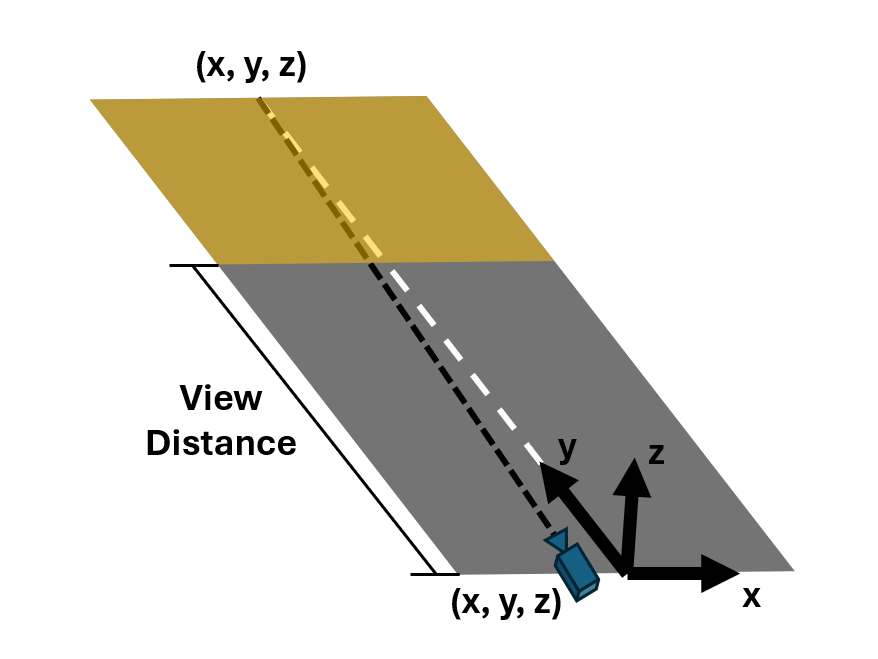
\includegraphics[width=0.45\linewidth]{figures/Camera Viewing.png}
    \caption{Diagram describing how the tasks handle the 'view distance' of the camera}
    \label{fig:ViewDist}
\end{figure}

%%%%%%%%%%%%%%%%%%%%%%%%%%
\section{Using EMG}
% Why am I even using EMG & what does it look like
Following the outline of the 

%%%%%%%%%%%%%%%%%%%%%%%%%%
\section{Completing the Task Construction}
As the code governing the task grew in volume and complexity it became clear that if progression were to continue a new approach was required to structure it in a more manageable form. This lead to the conversion of much of the written code to an object-orientated programming (OOP) style. While time consuming this involved the creation of a 'result' object which streamlined the data aquisition \& analysis immensely. This conversion to OOP was only made possible by previous examination of the structure \& formatting of the modelling code during the preliminary work for this thesis.

% Talk about patching all the edge cases/bugs here

%%%%%%%%%%%%%%%%%%%%%%%%%%
\section{Piloting the Trial and Gathering Data}

%%%%%%%%%%%%%%%%%%%%%%%%%%
\section{Task Flaws, Limitations \& Edge Cases}

%%%%%%%%%%%%%%%%%%%%%%%%%%
\section{Data Analysis}
\subsection{Reaction Times}
Taking the minimum reaction time to be 200ms the reaction time distribution was generated. \citep{jainComparativeStudyVisual2015}